% Created 2016-08-17 Wed 14:38
\documentclass[tikz]{standalone}

\usepackage[utf8]{inputenc}
\usepackage[T1]{fontenc}

\usepackage{circledsteps}

\RequirePackage{xcolor}

%% HPI color definitions according to the design manual
% These do not exactly match the RGB values used in the Powerpoint slide master due to unknown reasons
\definecolor{hpiyellow}{RGB}{246,168,0}
\definecolor{hpiorange}{RGB}{221,97,8}
\definecolor{hpired}{RGB}{177,6,58}
\definecolor{hpigray}{RGB}{90,96,101}
\definecolor{hpiblue}{RGB}{0,122,158}


\renewcommand{\sfdefault}{neosans}
% Different font weights for neosans
\newcommand{\textl}[1]{{\fontseries{l}\selectfont #1}} % light
\newcommand{\textm}[1]{{\fontseries{m}\selectfont #1}} % medium, same as default weight
\newcommand{\textsb}[1]{{\fontseries{sb}\selectfont #1}} % semibold
\newcommand{\textmb}[1]{{\fontseries{mb}\selectfont #1}} % bold, same as \textbf
\newcommand{\texteb}[1]{{\fontseries{eb}\selectfont #1}} % extra bold
\newcommand{\textub}[1]{{\fontseries{ub}\selectfont #1}} % ultra bold

\tikzset{every picture/.style={/utils/exec={\sffamily}}}
\tikzset{flipflop RSflanke/.style={
  flipflop,
  flipflop def={t1=S, t2=C, c2=1, t3=R, t6=Q, t4={\ctikztextnot{Q}}}
}}


\tikzset{
  mechanicalSwitch/.pic={
    \coordinate (-inUp) at (135:2); 
    \coordinate (-inDown) at (235:2);
    \coordinate (-out) at (2,0);
    \coordinate (-center) at (0,0);
    
    \draw (0,0) circle [radius = 2cm];
    \draw [fill=gray!20] (0,0) circle [radius = 0.2cm];

    \draw (0, 0) -- (2, 0);
    \draw (135:.8) -- (135:2); 
    \draw (225:.8) -- (225:2); 

    \draw [fill=gray!20] (2, 0) circle [radius=0.05cm]; 
    \draw [fill=gray!20] (135:2) circle [radius=0.05cm]; 
    \draw [fill=gray!20] (225:2) circle [radius=0.05cm]; 

    
    \draw [thick] (0,0) -- (175:1.5); 

    \draw [dashed, <->, domain=135:225] plot ({cos(\x)}, {sin(\x)}); 
  },
  mechanicalSwitchClosed/.pic={
    \coordinate (-inUp) at (135:2); 
    \coordinate (-inDown) at (255:2);
    \coordinate (-out) at (2,0);
    \coordinate (-center) at (0,0);
    \draw (0,0) circle [radius = 2cm];
    \draw [fill=gray!20] (0,0) circle [radius = 0.2cm];

    \draw (0, 0) -- (2, 0);
    \draw (135:.8) -- (135:2); 
    \draw (225:.8) -- (225:2); 

    \draw [fill=gray!20] (2, 0) circle [radius=0.05cm]; 
    \draw [fill=gray!20] (135:2) circle [radius=0.05cm]; 
    \draw [fill=gray!20] (225:2) circle [radius=0.05cm]; 

    
    \draw [thick] (0,0) -- (135:2); 

    \draw [dashed, <->, domain=135:225] plot ({cos(\x)}, {sin(\x)}); 
  }
}


\usetikzlibrary{calc}
\usetikzlibrary{positioning}


\usetikzlibrary{ext.positioning-plus,backgrounds}


\begin{document}

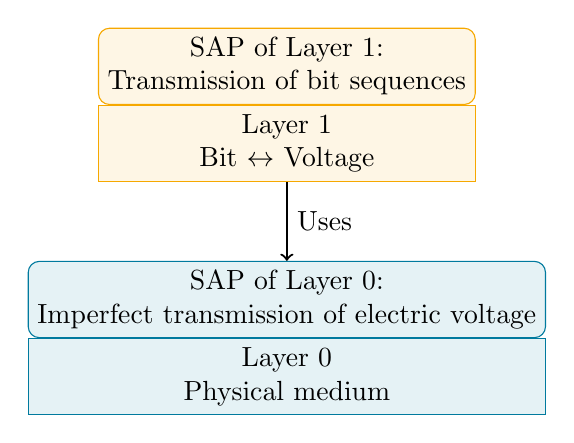
\begin{tikzpicture}
  \node[fill=hpiyellow!10, draw=hpiyellow, align=center, rounded corners] (sap1) {SAP of Layer 1:\\Transmission of bit sequences};
  \node[fill=hpiyellow!10, draw=hpiyellow, align=center, below=0 of -(sap1)] (l1) {Layer 1\\  Bit $\leftrightarrow$ Voltage };

  \node[fill=hpiblue!10, draw=hpiblue, align=center, rounded corners, below=of -(l1)] (sap0) {SAP of Layer 0:\\Imperfect transmission of electric voltage};
  \node[fill=hpiblue!10, draw=hpiblue, align=center, below=0 of -(sap0)] (l0) {Layer 0\\  Physical medium };


  \draw [->, thick] (l1) to node[right] {Uses} (sap0); 
\end{tikzpicture}


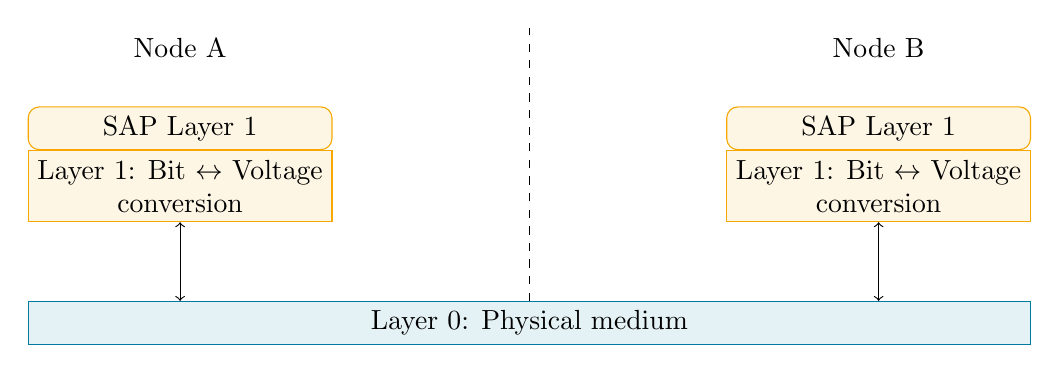
\begin{tikzpicture}
  \node[fill=hpiyellow!10, draw=hpiyellow, align=center,] (l1l)  {Layer 1: Bit $\leftrightarrow$ Voltage \\conversion}; 
  \node[fill=hpiyellow!10, draw=hpiyellow, align=center, rounded corners, above=0 of -(l1l)] (sap1l)  {SAP Layer 1};

  \node[fill=hpiyellow!10, draw=hpiyellow, align=center,right=5cm of l1l, ] (l1r)  {Layer 1: Bit $\leftrightarrow$ Voltage \\conversion}; 
  \node[fill=hpiyellow!10, draw=hpiyellow, align=center, rounded corners, above=0 of -(l1r)] (sap1r)  {SAP Layer 1}; 


  \node[fill=hpiblue!10, draw=hpiblue, below=1cm of -(l1l)(l1r)] (phy)  {Layer 0: Physical medium}; 


  \draw [<->] (l1l) -- (phy.north -| l1l); 
  \draw [<->] (l1r) -- (phy.north -| l1r); 

  \node [above=0.5 of sap1l] (nodeA) {Node A}; 
  \node [above=0.5 of sap1r] {Node B}; 
  
  \draw [dashed] (phy) -- (phy |- nodeA.north); 

  
\end{tikzpicture}

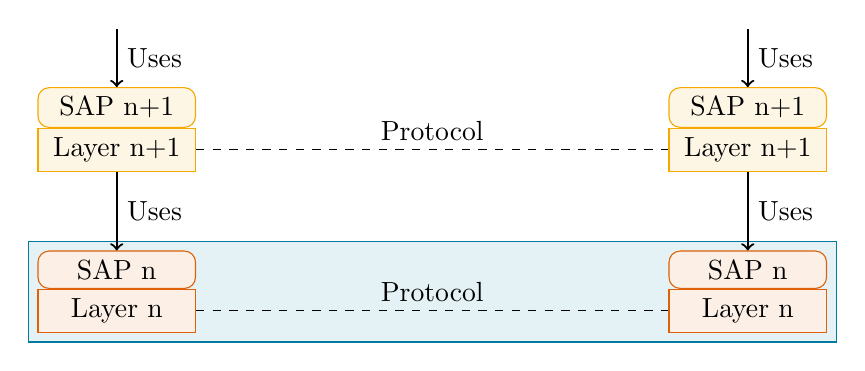
\begin{tikzpicture}
  \label{page:arch:saps_layers}

  \node[fill=hpiyellow!10, draw=hpiyellow, align=center, minimum width=2cm, rounded corners] (sap1l)  {SAP n+1};
  \node[fill=hpiyellow!10, draw=hpiyellow, align=center, below=0 of -(sap1l)] (l1l)  {Layer n+1}; 

  \node[fill=hpiyellow!10, draw=hpiyellow, align=center, minimum width=2cm, rounded corners, right=6cm of sap1l] (sap1r)  {SAP n+1}; 
  \node[fill=hpiyellow!10, draw=hpiyellow, align=center, below=0 of -(sap1r)] (l1r)  {Layer n+1}; 

  
  \node[fill=hpiorange!10, draw=hpiorange, align=center, minimum width=2cm, rounded corners, below=of l1l] (sap0l)  {SAP n};
  \node[fill=hpiorange!10, draw=hpiorange, align=center, below=0 of -(sap0l)] (l0l)  {Layer n}; 

  \node[fill=hpiorange!10, draw=hpiorange, align=center, minimum width=2cm, rounded corners, below=of l1r] (sap0r)  {SAP n}; 
  \node[fill=hpiorange!10, draw=hpiorange, align=center, below=0 of -(sap0r)] (l0r)  {Layer n}; 


  % \node[fill=hpiblue!10, draw=hpiblue, below=1cm of -(l1l)(l1r)] (phy)  {Layer 0: Physical medium}; 

  % \draw [<->] (l1l) -- (phy.north -| l1l); 
  % \draw [<->] (l1r) -- (phy.north -| l1r); 


  \draw [->, thick] (l1l) to node[right] {Uses} (sap0l); 
  \draw [->, thick] (l1r) to node[right] {Uses} (sap0r); 
  \draw [<-, thick] (sap1l) to node[right] {Uses} ++ (0,1); 
  \draw [<-, thick] (sap1r) to node[right] {Uses} ++ (0,1); 

  % \coordinate (tmp) at 
  % \draw [fill=hpiblue!10]   ($(sap0l)+(-1,0.5)$) -- (sap0r); 

  \begin{scope}[on background layer]
    \node [fill=hpiblue!10, draw=hpiblue, fit=(sap0l) (l0r) (sap0r) (l0l)] {}; 
  \end{scope}

  \draw [dashed] (l0l) to node[above] {Protocol} (l0r); 
  \draw [dashed] (l1l) to node[above] {Protocol} (l1r); 

\end{tikzpicture}


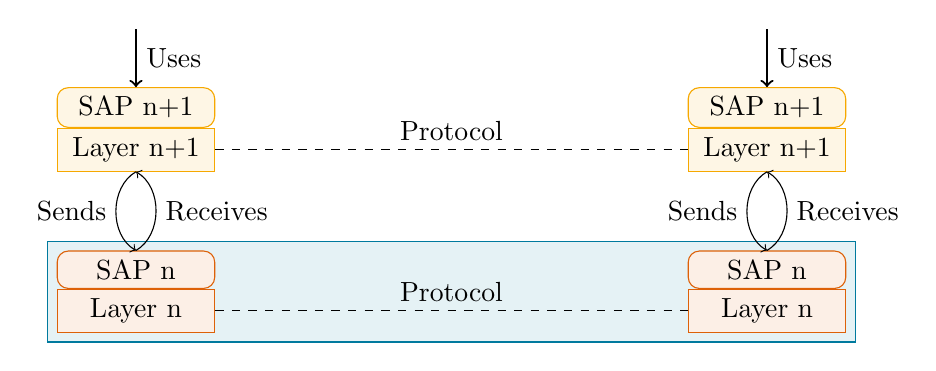
\begin{tikzpicture}
  \label{page:arch:layers:send_receive}

  \node[fill=hpiyellow!10, draw=hpiyellow, align=center, minimum width=2cm, rounded corners] (sap1l)  {SAP n+1};
  \node[fill=hpiyellow!10, draw=hpiyellow, align=center, below=0 of -(sap1l)] (l1l)  {Layer n+1}; 

  \node[fill=hpiyellow!10, draw=hpiyellow, align=center, minimum width=2cm, rounded corners, right=6cm of sap1l] (sap1r)  {SAP n+1}; 
  \node[fill=hpiyellow!10, draw=hpiyellow, align=center, below=0 of -(sap1r)] (l1r)  {Layer n+1}; 

  
  \node[fill=hpiorange!10, draw=hpiorange, align=center, minimum width=2cm, rounded corners, below=of l1l] (sap0l)  {SAP n};
  \node[fill=hpiorange!10, draw=hpiorange, align=center, below=0 of -(sap0l)] (l0l)  {Layer n}; 

  \node[fill=hpiorange!10, draw=hpiorange, align=center, minimum width=2cm, rounded corners, below=of l1r] (sap0r)  {SAP n}; 
  \node[fill=hpiorange!10, draw=hpiorange, align=center, below=0 of -(sap0r)] (l0r)  {Layer n}; 


  % \node[fill=hpiblue!10, draw=hpiblue, below=1cm of -(l1l)(l1r)] (phy)  {Layer 0: Physical medium}; 

  % \draw [<->] (l1l) -- (phy.north -| l1l); 
  % \draw [<->] (l1r) -- (phy.north -| l1r); 


  \draw [<-, thick] (sap1l) to node[right] {Uses} ++ (0,1); 
  \draw [<-, thick] (sap1r) to node[right] {Uses} ++ (0,1); 

  % \coordinate (tmp) at 
  % \draw [fill=hpiblue!10]   ($(sap0l)+(-1,0.5)$) -- (sap0r); 

  \begin{scope}[on background layer]
    \node [fill=hpiblue!10, draw=hpiblue, fit=(sap0l) (l0r) (sap0r) (l0l)] (l0) {}; 
  \end{scope}

  \draw [dashed] (l0l) to node[above] {Protocol} (l0r); 
  \draw [dashed] (l1l) to node[above] {Protocol} (l1r); 


  \draw [->] (l1l.south) to [out=210,in=150] node [left] {Sends} (l1l.south |- sap0l.north);
  \draw [->] (l1l.south |- sap0l.north) to [out=30,in=330]  node [right] {Receives} (l1l.south) ;


  \draw [->] (l1r.south) to [out=210,in=150] node [left] {Sends} (l1r.south |- sap0r.north);
  \draw [->] (l1r.south |- sap0r.north) to [out=30,in=330]  node [right] {Receives} (l1r.south) ;

  
\end{tikzpicture}

\end{document} 